\documentclass[12pt,a4paper]{article}

\usepackage[
    a4paper,
    top=3cm,
    bottom=3cm,
    left=4cm,
    right=3cm,
    columnsep=1.27cm,
    footskip=0.5cm
]{geometry}
\usepackage[T1]{fontenc}
\usepackage[utf8]{inputenc}
\usepackage{amsmath}
\usepackage{amsfonts}
\usepackage{amssymb}
\usepackage{newtxtext,newtxmath}
\usepackage{helvet}
\usepackage{setspace}
\usepackage{microtype}
\usepackage[round,authoryear]{natbib}
\usepackage{algorithmic}
\usepackage{graphicx}
\usepackage{textcomp}
\usepackage{caption}
\usepackage{titlesec}
\usepackage{dblfloatfix}
\usepackage[hidelinks,hypertexnames=false]{hyperref}
\usepackage{fancyhdr}

\usepackage{listings}
\usepackage{xcolor}
\usepackage{float}
\usepackage{array}
\usepackage{colortbl}
\usepackage{multirow}
\usepackage{booktabs}
\usepackage{url}
\usepackage{tikz}
\usetikzlibrary{positioning}
\usetikzlibrary{chains}
\usepackage{pgfplots}
\pgfplotsset{compat=1.18}

\newcommand{\Var}[2]{\gdef#1{#2}}
\input{config/settings}
\renewcommand{\judul}{Implementation and Evaluation of a Multi-Dimensional Resource Defragmentation Policy for the Kubernetes Descheduler}

\setlength{\parindent}{0.5in}
\setlength{\parskip}{0pt}
\setlength{\columnsep}{1.27cm}
\setlength{\headheight}{15pt}
\raggedbottom
\emergencystretch=2em

\titleformat{\section}
    {\normalfont\bfseries}
    {}
    {0pt}
    {\MakeUppercase}
\titleformat{\subsection}
    {\normalfont\bfseries}
    {}
    {0pt}
    {}
\titleformat{\subsubsection}
    {\normalfont\bfseries}
    {}
    {0pt}
    {}
\titlespacing*{\section}{0pt}{1.2\baselineskip}{0.4\baselineskip}
\titlespacing*{\subsection}{0pt}{0.9\baselineskip}{0.25\baselineskip}
\titlespacing*{\subsubsection}{0pt}{0.7\baselineskip}{0.2\baselineskip}

\captionsetup{
    font=small,
    labelfont=bf,
    labelsep=period,
    justification=centering
}

\lstset{
    basicstyle=\scriptsize\ttfamily,
    breaklines=true,
    breakatwhitespace=true,
    columns=fullflexible,
    keepspaces=true,
    showstringspaces=false,
    frame=single,
    captionpos=b,
    numbers=left,
    numberstyle=\tiny,
    xleftmargin=1.0em,
    framexleftmargin=0.6em,
    breakindent=0pt,
    postbreak=\mbox{\textcolor{gray}{$\hookrightarrow$}\space}
}

\let\cite\citep
\renewcommand{\refname}{References}

\fancypagestyle{uiarticle}{
    \fancyhf{}
    \fancyhead[R]{\thepage}
    \fancyfoot[R]{\fontsize{10}{12}\selectfont\sffamily\bfseries Universitas Indonesia}
    \renewcommand{\headrulewidth}{0pt}
    \renewcommand{\footrulewidth}{0pt}
}

\newcommand{\journalAuthors}{%
    \penulisDua, and Made Harta Dwijaksara%
}

\newcommand{\studentIdentityLines}{%
    \textbf{\penulisSatu~/ \npmSatu~/ \programSatu}\\
    \textbf{\penulisDua~/ \npmDua~/ \programDua}\\
    \textbf{\penulisTiga~/ \npmTiga~/ \programTiga}%
}

\newcommand{\frontHeading}[1]{%
    \begin{center}
        \bfseries\MakeUppercase{#1}
    \end{center}
}

\newcommand{\makeOuterCover}{%
    \begin{titlepage}
        \thispagestyle{empty}
        \begin{singlespace}
        \begin{center}
            
\includegraphics[width=2.5cm]{assets/pics/makara_kuning.png}\par
            \vspace{0.25cm}
            {\large\bfseries UNIVERSITAS INDONESIA\par}
            \vspace{1.0cm}
            {\large\bfseries\MakeUppercase{\judul}\par}
            \vspace{2.5cm}
            {\large\bfseries\MakeUppercase{\type}\par}
            \vspace{2.5cm}
            \studentIdentityLines\par
            \vfill
            {\large\bfseries
                FAKULTAS \MakeUppercase{\fakultas}\\
                PROGRAM STUDI \MakeUppercase{\programSatu}\\
                DEPOK\\
                \MakeUppercase{\bulanTahun}
            \par}
        \end{center}
        \end{singlespace}
    \end{titlepage}
}

\newcommand{\makeInnerTitlePage}{%
    \begin{titlepage}
        \thispagestyle{empty}
        \begin{singlespace}
        \begin{center}
            
\includegraphics[width=2.5cm]{assets/pics/makara_kuning.png}\par
            \vspace{0.25cm}
            {\large\bfseries UNIVERSITAS INDONESIA\par}
            \vspace{1.0cm}
            {\large\bfseries\MakeUppercase{\judul}\par}
            \vspace{2.2cm}
            {\large\bfseries\MakeUppercase{\type}\par}
            \vspace{0.5cm}
            Diajukan sebagai salah satu syarat untuk memperoleh gelar\\
            \gelar\par
            \vspace{2.0cm}
            \studentIdentityLines\par
            \vfill
            {\large\bfseries
                FAKULTAS \MakeUppercase{\fakultas}\\
                PROGRAM STUDI \MakeUppercase{\programSatu}\\
                DEPOK\\
                \MakeUppercase{\bulanTahun}
            \par}
        \end{center}
        \end{singlespace}
    \end{titlepage}
}

\newcommand{\makeOriginalityPage}{%
    \clearpage
    \thispagestyle{plain}
    \frontHeading{Halaman Pernyataan Orisinalitas}
    \vspace{1.8cm}
    \begin{center}
        \onehalfspacing
        \textbf{\type~ini adalah hasil karya kami sendiri,}\\
        \textbf{dan semua sumber baik yang dikutip maupun dirujuk}\\
        \textbf{telah kami nyatakan dengan benar.}

        \vspace{2.4cm}
        \begin{tabular}{l c l}
            \textbf{Nama Penulis 1} & : & \textbf{\penulisSatu}\\
            \textbf{NPM Penulis 1} & : & \textbf{\npmSatu}\\
            \textbf{Tanda Tangan Penulis 1} & : & \\
            &&\\[0.6cm]
            \textbf{Nama Penulis 2} & : & \textbf{\penulisDua}\\
            \textbf{NPM Penulis 2} & : & \textbf{\npmDua}\\
            \textbf{Tanda Tangan Penulis 2} & : & \\
            &&\\[0.6cm]
            \textbf{Nama Penulis 3} & : & \textbf{\penulisTiga}\\
            \textbf{NPM Penulis 3} & : & \textbf{\npmTiga}\\
            \textbf{Tanda Tangan Penulis 3} & : & \\
            &&\\[0.6cm]
            \textbf{Tanggal} & : & \textbf{\tanggalSiapSidang}\\
        \end{tabular}
    \end{center}
}

\newcommand{\makeApprovalPage}{%
    \clearpage
    \thispagestyle{plain}
    \frontHeading{Halaman Pengesahan}
    \vspace{0.4cm}
    \noindent\begin{tabular}{ll p{8.0cm}}
        \type~ini diajukan oleh & : & \\
        \textbf{Penulis 1} & & \\
        Nama & : & \penulisSatu\\
        NPM & : & \npmSatu\\
        Program Studi & : & \programSatu\\[0.15cm]
        \textbf{Penulis 2} & & \\
        Nama & : & \penulisDua\\
        NPM & : & \npmDua\\
        Program Studi & : & \programDua\\[0.15cm]
        \textbf{Penulis 3} & & \\
        Nama & : & \penulisTiga\\
        NPM & : & \npmTiga\\
        Program Studi & : & \programTiga\\[0.15cm]
        Judul \type & : & \judul\\
    \end{tabular}

    \vspace{0.7cm}
    \noindent\textbf{Telah berhasil dipertahankan di hadapan Dewan Penguji
    dan diterima sebagai bagian persyaratan yang diperlukan untuk memperoleh
    gelar \jenjang~pada Program Studi \programSatu, Fakultas \fakultas,
    Universitas Indonesia.}

    \vspace{0.7cm}
    \begin{center}
        \textbf{DEWAN PENGUJI}
    \end{center}

    \vspace{0.2cm}
    \begin{tabular}{l l p{6.6cm} l}
        Pembimbing & : & \pembimbingSatu & (\hspace{2.6cm})\\[0.35cm]
        Penguji & : & \pengujiSatu & (\hspace{2.6cm})\\[0.35cm]
        Penguji & : & \pengujiDua & (\hspace{2.6cm})\\
    \end{tabular}

    \vfill
    \begin{tabular}{ll l}
        Ditetapkan di & : & Depok\\
        Tanggal & : & \tanggalLulus\\
    \end{tabular}
}

\newcommand{\makePublicationApprovalPage}{%
    \clearpage
    \thispagestyle{plain}
    \frontHeading{Halaman Pernyataan Persetujuan Publikasi\\Tugas Akhir untuk Kepentingan Akademis}
    \vspace{0.4cm}
    \onehalfspacing
    \noindent Sebagai sivitas akademik Universitas Indonesia, kami yang bertanda
    tangan di bawah ini:

    \vspace{0.2cm}
    \noindent\begin{tabular}{p{3.4cm} l p{8.6cm}}
        \textbf{Penulis 1} & & \\
        Nama & : & \penulisSatu\\
        NPM & : & \npmSatu\\
        Program Studi & : & \programSatu\\[0.1cm]
        \textbf{Penulis 2} & & \\
        Nama & : & \penulisDua\\
        NPM & : & \npmDua\\
        Program Studi & : & \programDua\\[0.1cm]
        \textbf{Penulis 3} & & \\
        Nama & : & \penulisTiga\\
        NPM & : & \npmTiga\\
        Program Studi & : & \programTiga\\
        Fakultas & : & \fakultas\\
        Jenis karya & : & \type\\
    \end{tabular}

    \vspace{0.2cm}
    \noindent demi pengembangan ilmu pengetahuan, menyetujui untuk memberikan
    kepada Universitas Indonesia \textbf{Hak Bebas Royalti Noneksklusif
    (\textit{Non-exclusive Royalty Free Right})} atas karya ilmiah kami yang
    berjudul:

    \begin{center}
        \judul
    \end{center}

    \noindent beserta perangkat yang ada (jika diperlukan). Dengan Hak Bebas
    Royalti Noneksklusif ini Universitas Indonesia berhak menyimpan,
    mengalihmedia/formatkan, mengelola dalam bentuk pangkalan data
    (\textit{database}), merawat, dan memublikasikan tugas akhir kami selama
    tetap mencantumkan nama kami sebagai penulis/pencipta dan sebagai pemilik
    Hak Cipta.

    \vspace{0.2cm}
    \noindent Demikian pernyataan ini kami buat dengan sebenarnya.

    \vfill
    \begin{center}
        \begin{tabular}{lll}
            Dibuat di & : & Depok\\
            Pada tanggal & : & \tanggalSiapSidang\\
        \end{tabular}\\[0.4cm]
        Yang menyatakan

        \vspace{1.2cm}
        \begin{tabular}{ccc}
            (\penulisSatu) & (\penulisDua) & (\penulisTiga)
        \end{tabular}
    \end{center}
}

\newcommand{\abstractIndonesian}{%
Klaster Kubernetes yang dinamis mengakumulasi fragmentasi sumber daya
multidimensi yang menimbulkan kapasitas terdampar: CPU dan memori tersedia
secara agregat tetapi tersebar dalam bentuk yang tidak dapat dipakai oleh
\textit{Pod} baru. Penelitian ini menyajikan \textit{ResourceDefragmentation},
sebuah kebijakan \textit{Balance} pada Kubernetes Descheduler yang bekerja murni
berdasarkan \textit{request} sumber daya yang dideklarasikan, tanpa penggunaan
aktual. Kebijakan ini mengevaluasi bentuk penggunaan CPU-memori menggunakan
\textit{Resource Imbalance Index} (RII), \textit{Free-Space Index} (FSI), dan
\textit{bin score}, mengurutkan \textit{Node} sumber, lalu menggusur \textit{Pod}
yang \textit{Node} tujuan prediksinya memiliki \textit{bin score} proyeksi
tertinggi. \textit{Predictor} target penjadwal memastikan setiap penggusuran
memiliki tujuan yang layak, sementara batas utilisasi dan \textit{guard}
\textit{pack-upward} mencegah pengisian berlebih maupun perpindahan ke
\textit{Node} yang lebih kosong. Pada lima skenario sumber daya berbasis
\textit{request}, kebijakan ini mereklamasi empat \textit{Node} pada skenario
utilisasi rendah dan tiga \textit{Node} pada skenario terfragmentasi, sementara
\textit{HighNodeUtilization} tidak melakukan penggusuran sama sekali. Pada
skenario pengosongan heterogen, kebijakan menurunkan skor \textit{stranding}
dari 1,338 menjadi 0,123 (sekitar 91\%) hanya dengan dua penggusuran, sekaligus
mempertahankan atau meningkatkan \textit{headroom} penjadwalan yang seimbang.
Setiap eksekusi konvergen menuju \textit{pass} tanpa penggusuran tanpa
menyisakan \textit{Pod} berstatus \textit{Pending}. Secara keseluruhan, memilih
kandidat penggusuran berdasarkan keseimbangan \textit{Node} tujuan prediksinya
sudah cukup untuk mendorong reklamasi \textit{Node} dan defragmentasi
dimensional yang efektif.%
}

\newcommand{\abstractEnglish}{%
Dynamic Kubernetes clusters accumulate multi-dimensional resource fragmentation
that strands capacity: CPU and memory remain available in aggregate but scatter
into shapes that no single Node can offer to a new Pod. This study presents
\textit{ResourceDefragmentation}, a Kubernetes Descheduler \textit{Balance}
policy that operates purely on declared resource requests, without runtime
(actual) usage. The policy evaluates CPU-memory shape using the Resource
Imbalance Index (RII), Free-Space Index (FSI), and a density-and-balance bin
score, orders source Nodes, and evicts the Pod whose predicted scheduler target
has the highest projected bin score. A predicted-target check guarantees every
eviction has a feasible destination, while a utilization ceiling and a
pack-upward guard prevent overfilling a Node or relocating a workload to an
emptier one. Across five request-based resource scenarios, the policy reclaimed
four Nodes in the underutilized scenario and three Nodes in the fragmented
scenario, whereas \textit{HighNodeUtilization} performed no eviction at all. In
the heterogeneous-drain scenario, it reduced the cluster stranding score from
1.338 to 0.123 (about 91\%) with only two evictions, while preserving or
increasing balanced schedulability headroom. Every run converged to a
zero-eviction pass without leaving any Pod Pending. Overall, selecting eviction
candidates by the balance of their predicted landing Nodes is sufficient to
drive effective Node reclamation and dimensional defragmentation.%
}

\newcommand{\makeArticleAbstract}{%
    \clearpage
    \newgeometry{top=3cm,bottom=3cm,left=2.38cm,right=3cm}
    \pagenumbering{arabic}
    \setcounter{page}{1}
    \pagestyle{uiarticle}
    \singlespacing
    \begin{center}
        {\bfseries \judul\par}
        \vspace{0.6\baselineskip}
        {\journalAuthors\par}
        \vspace{0.25\baselineskip}
        {Program Studi \programSatu, Fakultas \fakultas, Universitas Indonesia\par}
    \end{center}

    \vspace{0.7\baselineskip}
    \frontHeading{Abstrak}
    \noindent\abstractIndonesian

    \vspace{0.5\baselineskip}
    \noindent\textit{Kata kunci: Kubernetes, Descheduler, Resource Defragmentation, Bin Packing Multidimensi, Reklamasi Node, Resource Imbalance Index}

    \vspace{0.9\baselineskip}
    \frontHeading{Abstract}
    \noindent\abstractEnglish

    \vspace{0.5\baselineskip}
    \noindent\textit{Keywords: Kubernetes, Descheduler, Resource Defragmentation, Multi-Dimensional Bin Packing, Node Reclamation, Resource Imbalance Index}
}

\begin{document}

% \makeOuterCover
% \pagenumbering{roman}
% \setcounter{page}{1}
% \makeInnerTitlePage
% \makeOriginalityPage
% \makeApprovalPage
% \makePublicationApprovalPage
\makeArticleAbstract

\clearpage
\newgeometry{
    top=3cm,
    bottom=3cm,
    left=2.22cm,
    right=2.11cm,
    columnsep=1.27cm
}
\twocolumn
\singlespacing
\pagestyle{uiarticle}

%----------------------------------------------------------------------------- %%
\section{Introduction}
\label{bab:1}
%----------------------------------------------------------------------------- %%

Kubernetes schedules Pods by filtering feasible Nodes and scoring the remaining alternatives. This process is effective for initial placement, but running Pods normally remain bound to their Nodes until they terminate or are recreated. As workloads scale and change, free CPU and memory can become scattered into incompatible shapes. Aggregate capacity may be sufficient while no individual Node can accommodate a new Pod, a condition commonly described as resource fragmentation.

Fragmentation affects schedulability, utilization, and infrastructure cost. A Node may retain CPU without enough memory, while another retains memory without enough CPU. These asymmetric residuals strand capacity because the two dimensions cannot be allocated independently~\cite{xiao2013dynamic,guo2025joint}. Directed Pod eviction can repair such placement states and reduce the number of Nodes required by the same workload~\cite{larsson_klein_elmroth_2023}.

The Kubernetes Descheduler provides a post-placement correction mechanism by evicting selected Pods and allowing the kube-scheduler to place their replacements~\cite{k8s_descheduler_docs}. For node reclamation, the important question is not merely whether a source Node is lightly utilized, but whether an evicted Pod has a feasible target that produces denser and better-shaped packing. This requires source-node assessment, target prediction, and an eviction budget that limits disruption. To remain mathematically aligned with the kube-scheduler, a defragmentation policy must evaluate Nodes primarily through their static declared resource requests rather than actual usage, because these static requests dictate placement feasibility and bin-packing shape.

This research develops \textit{ResourceDefragmentation}, a defragmentation-focused Descheduler \textit{Balance} policy that operates purely on declared CPU and memory requests. It identifies drain candidates using utilization and CPU-memory shape, orders them with a Resource Imbalance Index (RII) and Free-Space Index (FSI), predicts feasible scheduler targets, and chooses the Pod whose predicted landing Node has the strongest projected CPU-memory bin score. The kube-scheduler remains responsible for final binding.

This paper addresses the following research questions:

\begin{description}
    \item[\textbf{RQ1.}] How can a Descheduler policy identify and correct CPU-memory fragmentation through directed Pod eviction, and how effectively does it reclaim Nodes and reduce stranded capacity compared to a utilization-based baseline?
    \item[\textbf{RQ2.}] Does predicted-target, bin-score-based eviction-candidate selection improve packing quality and eviction efficiency relative to that baseline?
\end{description}

It makes the following contributions:

\begin{itemize}
    \item an implementation of \textit{ResourceDefragmentation} as a request-based \textit{Balance} plugin that repairs post-placement scatter without replacing the kube-scheduler;
    \item a Node-state model combining average utilization, a density-and-balance bin score, RII, and FSI to detect and order fragmented drain candidates; and
    \item a controlled evaluation across five node-reclamation and fragmentation scenarios, comparing the policy with the upstream \textit{HighNodeUtilization} strategy on node reclamation, dimensional stranding, schedulability headroom, and eviction cost.
\end{itemize}

%----------------------------------------------------------------------------- %%
\section{Literature Review}
\label{bab:2}
%----------------------------------------------------------------------------- %%

This section reviews the theoretical concepts and prior work that form the foundation of this study, including Kubernetes resource management, resource fragmentation, Descheduler mechanisms, and predicted-target eviction-candidate selection.

\subsection{Kubernetes Architecture and Resource Management}
\label{sec:kubernetesArchitecture}

Kubernetes distributes Pods across worker Nodes. For CPU and memory, a container may declare a resource request, a resource limit, both, or neither. Requests represent the resource baseline used by the scheduler when determining whether a Pod fits on a Node, whereas limits are runtime enforcement ceilings applied by the kubelet and container runtime~\cite{k8s_resource_management}. Kubernetes uses effective Pod requests when evaluating placement feasibility and resource allocation on each Node. Resource limits do not participate in this fit calculation; they define runtime enforcement ceilings after the Pod is running. Scheduler scoring strategies such as \textit{MostAllocated} and \textit{RequestedToCapacityRatio} may then use request-based allocation to favor denser packing~\cite{k8s_resource_bin_packing}.

Requests and limits also contribute to Pod Quality of Service (QoS) classification. A Pod is \textit{Guaranteed} when every container declares CPU and memory requests equal to its corresponding limits, while Pods with partial or unequal declarations are generally \textit{Burstable}. A Pod whose containers declare neither CPU nor memory requests or limits is \textit{BestEffort}~\cite{k8s_pod_qos}. If a limit is declared without a request, Kubernetes can use that limit as the effective request for the resource. A namespace \textit{LimitRange} may also assign default requests or limits during Pod admission. These defaults become part of the Pod's effective resource configuration~\cite{k8s_limit_range}.

These decisions are made when a Pod is scheduled. A running Pod is not continuously relocated when the cluster state changes, so an initially acceptable layout can become inefficient after scale-outs, terminations, and replacement events. This separation between initial placement and later cluster state motivates post-placement correction.

\subsection{Resource Fragmentation and Stranded Capacity}
\label{sec:resourceFragmentation}

Resource fragmentation occurs when free capacity is divided among Nodes in shapes that do not match incoming workloads. A cluster can have enough aggregate CPU and memory while no individual Node satisfies both dimensions of a Pod request. This makes CPU and memory placement a multi-dimensional problem rather than a scalar load-balancing problem.

CPU-memory skew is one source of stranded capacity. If one Node is CPU-heavy and another is memory-heavy, each leaves a different residual resource that cannot be consumed alone. The absolute difference between normalized CPU and memory fractions provides a direct shape indicator, while the product of free CPU and memory fractions represents the jointly usable free-space region. Prior work shows that directed eviction can repair fragmented Kubernetes layouts and support Node reclamation~\cite{larsson_klein_elmroth_2023}.

\subsection{Resource Defragmentation and Multi-Resource Bin Packing}
\label{sec:binPacking}

Resource packing seeks to place workloads on fewer active Nodes so that empty Nodes can be removed or powered down. In a multi-resource setting, dense packing alone is insufficient: a target can be highly utilized but badly skewed. A useful packing score should therefore represent both density and CPU-memory balance. Container resource defragmentation and task scheduling have been studied using optimization and learning-based methods~\cite{guo2025joint,bagaa2024multiobjective}, but these are commonly oriented toward placement or scheduling decisions rather than long-term post-placement correction in Kubernetes clusters.

The policy in this research uses normalized CPU and memory fractions. Average utilization represents density, while a bin score combines density with the absolute distance between the two dimensions. The Resource Imbalance Index (RII) preserves the direction of skew, and the Free-Space Index (FSI) measures the rectangular CPU-memory headroom. Together these quantities identify Nodes that are lightly loaded, poorly shaped, or under pressure from a narrow free-space region.

\subsection{Kubernetes Descheduler}
\label{sec:deschedulerLimitations}

The Kubernetes Descheduler evicts Pods that violate a policy or contribute to an undesirable placement state, after which normal controllers recreate the Pods and kube-scheduler places them again~\cite{k8s_descheduler_docs}. It provides an appropriate extension point for node reclamation because it can repair placement without modifying the scheduler.

An eviction policy must nevertheless account for the scheduler boundary. Deleting a Pod does not guarantee that it moves to a useful Node; it may become Pending, return to its origin, or land on a target that worsens fragmentation. A node reclamation-oriented policy therefore benefits from predicting feasible non-origin targets and rejecting movements that exceed a configured ceiling or pack downward.

Upstream utilization policies provide important baselines. \textit{HighNodeUtilization} packs by draining low-utilization Nodes toward more utilized Nodes, but it does not explicitly optimize CPU-memory stranding. This distinction is central to the evaluation in Section~\ref{bab:4}.

\subsection{Predicted-Target Eviction-Candidate Selection}
\label{sec:predictedTargetSelection}

Eviction-candidate selection can be formulated around the expected landing state. For every evictable Pod on a drain candidate, \textit{predictSchedulerTarget} simulates request-based placement on non-origin Nodes that satisfy scheduler constraints. Feasible targets must have sufficient CPU and memory, remain below a node reclamation ceiling after placement, and be at least as packed as the source.

The target with the best projected CPU-memory bin score is retained for each Pod. The Pod whose predicted target has the highest score is selected for eviction. This single criterion aligns the action directly with the desired destination state: the selected movement should place complementary resource shapes together while preserving node reclamation pressure.

\subsection{Current Approaches and Research Gap}
\label{sec:researchGap}

Existing mechanisms address individual parts of the problem. Scheduler scoring improves new placement, utilization-based descheduling drains Nodes according to thresholds, and fragmentation research motivates directed eviction. The remaining gap is a practical Descheduler policy that combines:

\begin{itemize}
    \item source assessment using utilization and CPU-memory shape;
    \item RII/FSI-based drain ordering;
    \item request-feasible scheduler-target prediction;
    \item a direct projected-target balance criterion; and
    \item bounded, convergent eviction.
\end{itemize}

\textit{ResourceDefragmentation} is designed to fill this gap while leaving final binding to the standard kube-scheduler.

%----------------------------------------------------------------------------- %%
\section{Policy Design and Implementation}
\label{bab:3}
%----------------------------------------------------------------------------- %%

This section presents the design and implementation of \textit{ResourceDefragmentation}, a \textit{Balance} plugin for post-placement consolidation in the Kubernetes Descheduler. It builds a snapshot of worker Nodes based on Pod resource requests, finds source Nodes that are either sparse or poorly shaped in CPU-memory space, predicts feasible landing Nodes for their Pods, and evicts the Pod whose predicted scheduler target has the strongest projected CPU-memory bin score. The kube-scheduler remains responsible for final binding.

The experimental configuration explicitly uses declared Pod requests. This keeps Node assessment, feasibility checks, and target prediction aligned with the admission model used by kube-scheduler, and it deliberately excludes runtime (actual) usage so that placement feasibility and bin-packing shape drive every decision.

\subsection{System Overview}
\label{sec:defrag_system_overview}

Figure~\ref{fig:defrag_highlevel} shows the end-to-end control flow of the \textit{ResourceDefragmentation} plugin, from the entry point of the Descheduler \textit{Balance} function to the eviction decision. The plugin operates in two phases: an assessment-and-ordering phase that builds the drain-candidate set, and a bounded eviction loop that relocates Pods from those candidates.

In the first phase, the plugin scans every worker Node. Control-plane Nodes are skipped, and for each remaining Node it computes the average utilization and bin score. A Node whose average utilization and bin score both stay at or above the drain threshold is well-packed and is skipped; otherwise the Node is scored with its Resource Imbalance Index (RII), Free-Space Index (FSI), and priority \(P_n\), added to the drain-candidate set, and the set is sorted in descending priority.

In the second phase, the plugin iterates over the ordered candidates. The loop stops once the per-sweep eviction budget is reached. A Node already marked as a bin, that is, a recent eviction target, is skipped so the same sweep does not drain a Node it has just packed. Otherwise the plugin selects the Pod whose predicted scheduler target has the highest projected bin score; if a feasible target exists the Pod is evicted and the local cache and bin set are updated, and if not the Node is skipped. The remaining subsections formalize each stage: Section~\ref{sec:defrag_node_metrics} defines the Node-state metrics, Section~\ref{sec:defrag_drain_candidates} the drain-candidate detection and ordering, Section~\ref{sec:defrag_target_prediction} the predicted scheduler target, and Section~\ref{sec:defrag_victim_selection} the eviction-candidate selection.

\begin{figure*}[tbp]
    \centering
    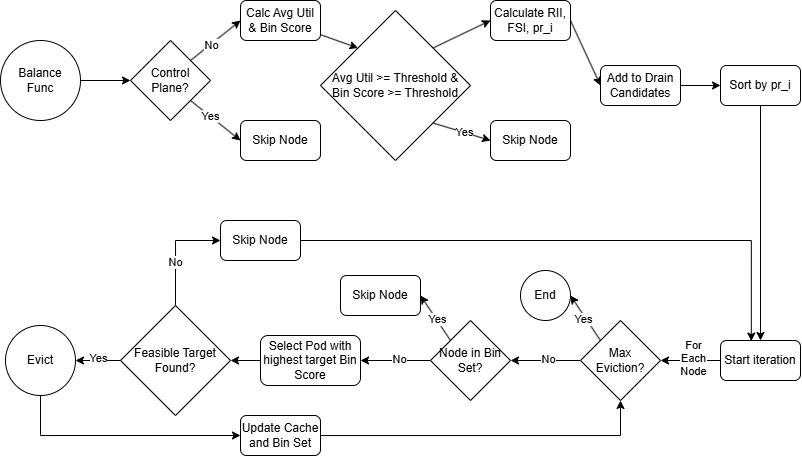
\includegraphics[width=0.95\textwidth]{assets/pics/defrag/highlevel_defrag.png}
    \caption{High-level control flow of the \textit{ResourceDefragmentation} plugin, from Node assessment and drain-candidate ordering to the bounded predicted-target eviction loop.}
    \label{fig:defrag_highlevel}
\end{figure*}

\subsection{Node-State Metrics}
\label{sec:defrag_node_metrics}

For Node \(n\), let \(u_{n,c}\) and \(u_{n,m}\) denote normalized requested CPU and memory:

\[
    u_{n,c} = \frac{R_{n,c}}{C_{n,c}},
    \qquad
    u_{n,m} = \frac{R_{n,m}}{C_{n,m}},
\]

where \(u_{n,c}\) is the normalized CPU utilization of Node \(n\), \(u_{n,m}\) is the normalized memory utilization of Node \(n\), \(R_{n,c}\) is the sum of CPU requests from all Pods on Node \(n\), \(R_{n,m}\) is the sum of memory requests from all Pods on Node \(n\), \(C_{n,c}\) is the allocatable CPU capacity of Node \(n\), and \(C_{n,m}\) is the allocatable memory capacity of Node \(n\). Average utilization represents density:

\[
    U_n^{avg} = \frac{u_{n,c} + u_{n,m}}{2},
\]

where \(U_n^{avg}\) is the average utilization of Node \(n\), representing overall resource density by taking the mean of normalized CPU and memory utilization.

The bin score is a custom composite scoring function derived from the standard multi-dimensional bin-packing heuristics used in the Kubernetes scheduling plugins~\cite{k8s_resource_bin_packing}. It fuses two signals that those plugins apply separately, namely the density preference of the \texttt{MostAllocated} strategy, which favors well-filled Nodes, and the per-dimension balance preference of the \texttt{BalancedAllocation} strategy, which penalizes Nodes whose CPU and memory utilization diverge. Combining density and dimensional balance into a single quantity yields

\[
    B_n =
    \frac{
        \frac{u_{n,c}+u_{n,m}}{2}
        \left(1-\left|u_{n,c}-u_{n,m}\right|\right)
    }{2},
\]

where \(B_n\) is the bin score of Node \(n\). The first factor \(\tfrac{u_{n,c}+u_{n,m}}{2}\) is the density term inherited from \texttt{MostAllocated}, while the penalty factor \(1-|u_{n,c}-u_{n,m}|\) is the balance term inherited from \texttt{BalancedAllocation}, which reduces the score when CPU and memory utilization diverge. A dense and balanced Node therefore has a high \(B_n\), whereas an empty or strongly skewed Node has a lower score. The signed Resource Imbalance Index, adapted to normalized request fractions from the server imbalance index of \cite{guo2025joint}, identifies the skew direction:

\[
    RII_n = u_{n,c} - u_{n,m},
\]

where \(RII_n\) is the Resource Imbalance Index of Node \(n\). A positive value indicates CPU-heavy skew (CPU utilization exceeds memory utilization), while a negative value indicates memory-heavy skew. The Free-Space Index, adapted from the free-space size index of \cite{guo2025joint} by expressing the headroom in normalized rather than absolute units, represents joint CPU-memory headroom:

\[
    FSI_n = (1-u_{n,c})(1-u_{n,m}),
\]

where \(FSI_n\) is the Free-Space Index of Node \(n\), representing the product of remaining CPU capacity \((1-u_{n,c})\) and remaining memory capacity \((1-u_{n,m})\). A higher \(FSI_n\) indicates a larger jointly usable headroom region, while a low \(FSI_n\) suggests constrained free space in at least one dimension.

\subsection{Drain-Candidate Detection and Ordering}
\label{sec:defrag_drain_candidates}

A worker Node with at least one evictable Pod becomes a drain candidate when either its average utilization or its bin score is below the configured drain threshold \(\tau\):

\[
    U_n^{avg} < \tau
    \quad \lor \quad
    B_n < \tau.
\]

The disjunction allows the policy to act on two resource-only states. A lightly utilized but balanced Node can be drained to free infrastructure, while a more utilized but badly skewed Node can be drained because its remaining headroom is hard to reuse.

Drain candidates are processed in descending priority:

\[
    P_n =
    0.5\left|RII_n\right|
    +
    0.5\frac{1}{FSI_n+1\mathrm{e}{-}10}.
\]

The first term emphasizes dimensional skew. The second term emphasizes a narrow jointly usable free-space region. Following the priority formulation of \cite{guo2025joint}, the constant is fixed at \(1\mathrm{e}{-}10\) and is added to the free-space term of \emph{every} Node as a numerical guard against division by zero, rather than being applied conditionally only when \(FSI_n = 0\). Because \(1\mathrm{e}{-}10\) is negligible relative to any non-zero \(FSI_n \in (0,1]\), it leaves the relative ordering of drain candidates unchanged for partially loaded Nodes, while bounding the term to a large finite value of \(1\mathrm{e}{+}10\) when a Node has no jointly usable headroom (\(FSI_n = 0\)), so that fully constrained Nodes receive the highest priority. Utilization and bin score decide whether a Node enters the drain set, while RII and FSI decide which drain candidate is handled first.

The two weights of \(0.5\) generalize the priority formulation of \cite{guo2025joint}, which writes the priority as \(w_p\left|RII_n\right| + (1-w_p)\,/(FSI_n+\epsilon)\) for a tunable weight \(w_p\). Setting \(w_p = 0.5\) treats dimensional skew and free-space scarcity as co-equal fragmentation signals, so that neither criterion is privileged a priori in the absence of a workload-specific reason to favor one. The two terms nonetheless occupy different numeric ranges: \(\left|RII_n\right| \in [0,1]\), whereas \(1/(FSI_n+1\mathrm{e}{-}10) \in [1,\,1\mathrm{e}{+}10]\). The free-space term therefore dominates the ordering for densely packed Nodes that have little joint headroom, while \(\left|RII_n\right|\) acts as a secondary, skew-based tie-breaker among Nodes with comparable free space.

Adjusting this weighting does not change the descheduler as a whole. The priority \(P_n\) governs only the \emph{order} in which already-selected drain candidates are processed; it does not decide which Nodes enter the drain set, whether a predicted target is feasible, the pack-upward guard, the utilization ceiling, or the bounded convergence loop. Re-weighting therefore alters the drain trajectory, namely which Node is handled first and possibly the number of passes required, and can shift the final layout only at the margin, for instance when the pass budget is exhausted before convergence. Because every pass re-evaluates the cluster state and the loop terminates only when a pass produces zero evictions, the policy's feasibility, safety, and convergence properties are independent of \(w_p\), and the converged layout remains stable across reasonable weightings. The weight is thus a tuning knob for ordering and efficiency rather than a parameter that redefines what the descheduler is permitted to evict.

\subsection{Predicted Scheduler Target}
\label{sec:defrag_target_prediction}

For every evictable Pod \(p\) on source Node \(s\), the plugin examines each non-origin worker Node as a potential relocation target. Let \(r_{p,c}\) and \(r_{p,m}\) denote the CPU and memory requests of \(p\). Placing \(p\) on a target Node \(t\) yields the projected utilization

\[
    u'_{t,c} = \frac{R_{t,c} + r_{p,c}}{C_{t,c}},
    \qquad
    u'_{t,m} = \frac{R_{t,m} + r_{p,m}}{C_{t,m}}.
\]

A non-origin Node \(t\) is admissible only if it is schedulable and \(p\) tolerates its taints. An admissible Node is a feasible target when it additionally satisfies the request-fit, utilization-ceiling, and pack-upward conditions, respectively:

\[
\begin{array}{@{}l@{}}
    R_{t,c} + r_{p,c} \leq C_{t,c},\quad
    R_{t,m} + r_{p,m} \leq C_{t,m},\\
    u'_{t,c} \leq \theta,\quad
    u'_{t,m} \leq \theta,\\
    \min\!\left(u'_{t,c}, u'_{t,m}\right)
    \geq \min\!\left(u_{s,c}, u_{s,m}\right).
\end{array}
\]

where \(\theta\) is the configured target-utilization ceiling, and \(u_{s,c}\) and \(u_{s,m}\) are the current CPU and memory utilization of source Node \(s\). The request-fit condition ensures that the projected requests do not exceed allocatable capacity in either dimension. The utilization-ceiling condition caps the projected utilization so that consolidation does not overload a target. The pack-upward guard requires the least-utilized dimension of the target to be at least as loaded as the least-utilized dimension of the source, which prevents an eviction from merely relocating a Pod to an emptier Node.

Let \(\mathcal{F}(p)\) denote the set of all feasible targets for \(p\). The function \textit{predictSchedulerTarget} returns the feasible Node that maximizes the projected bin score after receiving \(p\):

\[
    t_p = \operatorname*{arg\,max}_{t \in \mathcal{F}(p)} B'_t,
\]

where \(B'_t\) is the bin score \(B_t\) evaluated under the projected utilization \(\left(u'_{t,c}, u'_{t,m}\right)\). If \(\mathcal{F}(p) = \varnothing\), Pod \(p\) has no feasible target and is not evicted.

\subsection{Predicted-Target Eviction-Candidate Selection}
\label{sec:defrag_victim_selection}

For candidate Pod \(p\), let \(t_p\) be its predicted target and \(B'_{t_p}\) the target bin score after placement. The selected eviction candidate is:

\[
    p^\star = \arg\max_{p} B'_{t_p}.
\]

This is the only eviction-candidate selection criterion after target feasibility is checked. It directly prefers a movement that produces the best projected CPU-memory shape at the expected destination. Candidates without a feasible target are excluded. After a successful eviction, the local source and predicted-target snapshots are updated before the next decision. Predicted targets are marked as bins so the same pass does not subsequently drain a Node that has just received packed workload.

Appendix~\ref{appendix:resource_defrag} summarizes the complete execution flow.

\subsection{Plugin Configuration}
\label{sec:resource_defrag_config}

\begin{table*}[tbp]
    \centering
    \caption{ResourceDefragmentation Plugin Arguments}
    \label{tab:resource_defrag_args}
    \renewcommand{\arraystretch}{1.25}
    \resizebox{\textwidth}{!}{%
    \begin{tabular}{l l l p{7.0cm}}
        \hline
        \textbf{Parameter} & \textbf{Type} & \textbf{Experiment} & \textbf{Purpose} \\
        \hline
        \textit{maxEvictions} & integer & \(50\) & Upper bound on successful eviction attempts in one pass. \\
        \textit{consolidationThreshold} & float & \(0.40\) & Marks a Node as a drain candidate when average utilization or bin score is below this value. \\
        \textit{consolidationTarget} & float & \(0.90\) & Maximum projected CPU or memory utilization on a target Node. \\
        \textit{usageMode} & string & \textit{requests} & Pins the experiment to declared requests so all compared policies use the same signal. \\
        \textit{namespaces} & object & exclude system & Restricts candidate Pods and excludes infrastructure namespaces. \\
        \hline
    \end{tabular}%
    }
\end{table*}

\begin{figure*}[tbp]
    \centering
    \begin{minipage}{0.95\textwidth}
    \lstinputlisting[
        caption={Request-based ResourceDefragmentation configuration using the ResourceDefragmentationC2 plugin.},
        label={lst:resource_defrag_config_requests},
    ]{assets/codes/pseudos/resource-defrag-config-requests.psu}
    \end{minipage}
\end{figure*}

%-----------------------------------------------------------------------------%
\section{Experiment and Evaluation}
\label{bab:4}
%-----------------------------------------------------------------------------%

This section evaluates \textit{ResourceDefragmentation} against the upstream \textit{HighNodeUtilization} strategy across five node-reclamation and fragmentation scenarios, using request-space Node state throughout so that placement feasibility and CPU-memory shape, rather than runtime telemetry, drive every comparison.

\subsection{Experimental Setup}
\label{sec:defrag_experimental_setup}

The experiment uses one control-plane Node and six worker Nodes. Each worker provides \(2000\,m\) allocatable CPU and approximately \(811\,Mi\) allocatable memory. Pause containers reserve declared requests while contributing negligible runtime load, allowing the experiment to control the request-space layout precisely.

The scheduler uses \textit{MostAllocated} and \textit{BalancedAllocation}. Both policies operate on identical initial workloads and namespace scope. System workloads are excluded from eviction. The drain threshold is \(0.40\), the target-utilization ceiling is \(0.90\), each scenario permits at most five Descheduler passes, and every policy-scenario cell is repeated with three seeds.

The two systems under comparison are:

\begin{itemize}
    \item \textbf{HighNodeUtilization (HNU):} the upstream utilization-based baseline with CPU and memory thresholds of \(40\%\).
    \item \textbf{ResourceDefragmentation (RD):} the proposed resource-only policy using request-based Node state, RII/FSI-based source ordering, \textit{predictSchedulerTarget}, and projected target bin score as its eviction-candidate criterion.
\end{itemize}

\subsection{Scenarios}
\label{sec:defrag_scenarios}

\begin{table*}[tbp]
    \centering
    \caption{ResourceDefragmentation Evaluation Scenarios}
    \label{tab:defrag_scenarios}
    \small
    \renewcommand{\arraystretch}{1.2}
    \begin{tabular}{l p{3.6cm} p{7.4cm}}
        \hline
        \textbf{Scenario} & \textbf{Intent} & \textbf{Initial condition} \\
        \hline
        S1 & Pure node reclamation & Uniformly underutilized Nodes whose workloads can be packed onto fewer workers. \\
        S2 & Reducible stranding & Complementary CPU-heavy and memory-heavy Nodes with no clearly high-utilization target. \\
        S3 & Mixed objective & Underutilized drain Nodes coexist with already dense balanced Nodes. \\
        S4 & Hogs and jumbo Pod & Skewed resource hogs must be merged around a large workload. \\
        S5 & Heterogeneous drain & A drain Node contains differently shaped Pods that should land on complementary targets. \\
        \hline
    \end{tabular}
\end{table*}

S1 primarily tests Node reclamation. S2 and S4 test whether dimensional fragmentation can be reduced when a scalar utilization baseline has no suitable action. S3 combines node reclamation and shape preservation. S5 isolates shape-aware eviction-candidate selection during a heterogeneous drain.

\subsection{Evaluation Metrics}
\label{sec:defrag_metrics}

The success of each policy-scenario cell is assessed through five complementary metrics that jointly capture node reclamation, dimensional balance, residual schedulability, and operational cost. Every metric operates on request-space Node state, so the cluster layout is described entirely by per-Node resource requests rather than runtime telemetry. The fundamental quantity shared by all metrics is the per-dimension utilization fraction of a worker Node \(n\):

\[
u_{n,R}
=
\frac{R_{\text{req}}(n)}
{R_{\text{alloc}}(n)},
\qquad
R \in \{\text{cpu}, \text{mem}\}
\]

Where:

\begin{itemize}
    \item \(u_{n,R}\) is the request-based utilization fraction of Node \(n\) along dimension \(R\), bounded in \([0,1]\).

    \item \(R_{\text{req}}(n)\) is the sum of resource \(R\) requested by all evictable experiment Pods assigned to Node \(n\).

    \item \(R_{\text{alloc}}(n)\) is the allocatable capacity of Node \(n\) for resource \(R\) (\(2000\,m\) CPU and approximately \(811\,Mi\) memory per worker).
\end{itemize}

%-----------------------------------------------------------------------------%
\paragraph{Active Node Count}
\label{subsubsec:defrag_metric_active}
%-----------------------------------------------------------------------------%
The Active Node Count (\(N_{\text{active}}\)) is the primary indicator of node reclamation. A worker Node is counted as active only when it hosts at least one evictable experiment workload; infrastructure namespaces such as \textit{kube-system} are excluded and therefore never keep a Node active.

\[
N_{\text{active}}
=
\sum_{n=1}^{N} a_n
\]

\[
a_n =
\begin{cases}
1, & \text{if } \sum R_{\text{req}}(n) > 0 \\
0, & \text{otherwise}
\end{cases}
\]

Where:

\begin{itemize}
    \item \(N_{\text{active}}\) is the number of worker Nodes hosting evictable experiment workloads.

    \item \(a_n\) is the binary activity indicator for Node \(n\).

    \item \(N\) is the total number of worker Nodes available in the scenario.
\end{itemize}

A reduction in \(N_{\text{active}}\) between the before- and after-snapshots indicates that one or more Nodes have been fully drained and become reclaimable for scale-down. This metric directly measures the consolidation objective and is reported as the before-and-after pair together with the number of Nodes reclaimed.

%-----------------------------------------------------------------------------%
\paragraph{Resource Stranding Score}
\label{subsubsec:defrag_metric_stranding}
%-----------------------------------------------------------------------------%
Because defragmentation optimizes the geometric \emph{shape} of utilization rather than its absolute spread, the cluster is evaluated through a stranding score that measures how far each Node deviates from per-dimension balance. The cluster stranding score \(S\) aggregates the absolute CPU-to-memory imbalance across all active Nodes:

\[
    S = \sum_{n \in N_{\text{active}}} \left|u_{n,\text{cpu}} - u_{n,\text{mem}}\right|.
\]

Where:

\begin{itemize}
    \item \(S\) is the cluster-wide resource stranding score.

    \item \(u_{n,\text{cpu}}\) and \(u_{n,\text{mem}}\) are the request-based CPU and memory utilization fractions of Node \(n\).
\end{itemize}

A Node with a large gap between its CPU and memory fractions strands the under-used dimension, since the remaining capacity cannot be allocated to a balanced reference workload. A lower \(S\) therefore indicates that CPU and memory fractions are more tightly aligned across the cluster, unlocking trapped capacity. Unlike a global standard deviation, \(S\) is insensitive to intentional differences in absolute load between Nodes and reacts only to per-Node dimensional skew.

%-----------------------------------------------------------------------------%
\paragraph{Average Active-Node Utilization}
\label{subsubsec:defrag_metric_density}
%-----------------------------------------------------------------------------%
To quantify packing density, the Average Active-Node Utilization (\(\bar{U}\)) reports the mean request-based load of the Nodes that remain active after descheduling, averaged over both resource dimensions:

\[
\bar{U}
=
\frac{1}{N_{\text{active}}}
\sum_{n : a_n = 1}
\frac{u_{n,\text{cpu}} + u_{n,\text{mem}}}{2}
\times 100\%
\]

Where:

\begin{itemize}
    \item \(\bar{U}\) is the average utilization of the surviving active Nodes, expressed as a percentage.

    \item \(N_{\text{active}}\) is the number of active Nodes after descheduling.

    \item \(\frac{u_{n,\text{cpu}} + u_{n,\text{mem}}}{2}\) is the mean per-dimension utilization fraction of Node \(n\).
\end{itemize}

A higher \(\bar{U}\) indicates that the surviving Nodes carry denser workloads, which is the expected consequence of successful consolidation. This metric complements \(N_{\text{active}}\): reclaiming Nodes is only beneficial when the retained Nodes absorb the displaced load rather than leaving the cluster uniformly sparse.

%-----------------------------------------------------------------------------%
\paragraph{Balanced Headroom}
\label{subsubsec:defrag_metric_headroom}
%-----------------------------------------------------------------------------%
The Balanced Headroom (\(H_{balanced}\)) converts residual request space into a schedulability-oriented quantity. It counts how many reference Pods, each requesting \(200\,m\) CPU and \(80\,Mi\) memory, can still be placed across the cluster after descheduling. Let \(A_{\text{cpu}}(n)\) and \(A_{\text{mem}}(n)\) denote the remaining requested CPU and memory space on Node \(n\):

\[
\begin{aligned}
H_{balanced}
&=
\sum_{n=1}^{N}
\min\!\Biggl(
\left\lfloor
\frac{A_{\text{cpu}}(n)}{c_{\text{ref}}}
\right\rfloor,\\
&\qquad\qquad
\left\lfloor
\frac{A_{\text{mem}}(n)}{m_{\text{ref}}}
\right\rfloor
\Biggr)
\end{aligned}
\]

Where:

\begin{itemize}
    \item \(H_{balanced}\) is the total number of \(200\,m/80\,Mi\) reference Pods that fit in the remaining request space.

    \item \(c_{\text{ref}} = 200\,m\) and \(m_{\text{ref}} = 80\,Mi\) are the CPU and memory requests of the balanced reference Pod.

    \item the per-Node \(\min(\cdot)\) enforces that a reference Pod fits only when both dimensions admit it, penalizing Nodes whose free capacity is stranded on a single axis.
\end{itemize}

A higher \(H_{balanced}\) indicates that defragmentation has reassembled fragmented free capacity into contiguous, jointly schedulable space. Because the per-Node term is limited by the tighter dimension, a Node with abundant free CPU but little free memory contributes little headroom, which is precisely the stranding that the policy aims to remove.

The same construction generalizes to any reference Pod shape \(r = (c_r, m_r)\), giving a family of probes \(H_r\) that reveal \emph{which} kind of capacity a layout can still admit:

\[
\begin{aligned}
H_r
&=
\sum_{n=1}^{N}
\min\!\Biggl(
\left\lfloor
\frac{A_{\text{cpu}}(n)}{c_r}
\right\rfloor,\\
&\qquad\qquad
\left\lfloor
\frac{A_{\text{mem}}(n)}{m_r}
\right\rfloor
\Biggr)
\end{aligned}
\]

In addition to the balanced probe, three skewed probes are evaluated: a CPU-skewed Pod (\(H_{cpu\text{-}skewed}\)), a memory-skewed Pod (\(H_{mem\text{-}skewed}\)), and a large jumbo Pod (\(H_{jumbo}\), \(800\,m/324\,Mi\)). The balanced probe measures general schedulability, the two skewed probes measure how much single-axis capacity remains usable, and the jumbo probe measures whether the layout retains room for large indivisible workloads. Together they show that defragmentation does not merely free aggregate space but free space of the right shape.

%-----------------------------------------------------------------------------%
\paragraph{Eviction Count and Efficiency}
\label{subsubsec:defrag_metric_eviction}
%-----------------------------------------------------------------------------%
The Eviction Count (\(E_{count}\)) measures the operational cost of a descheduling sweep as the total number of Pods relocated, extracted from the Descheduler job log:

\[
E_{count}
=
\sum_{j \in J} e_j
\]

Where:

\begin{itemize}
    \item \(E_{count}\) is the total number of Pods evicted across all passes of a sweep.

    \item \(J\) is the set of log entries recorded during the job lifecycle.

    \item \(e_j\) is a binary flag equal to \(1\) when log entry \(j\) records an eviction, and \(0\) otherwise.
\end{itemize}

Efficiency is interpreted jointly from \(E_{count}\), the number of Nodes reclaimed (\(\Delta N_{\text{active}}\)), and the reduction in stranding (\(\Delta S\)). A policy is more efficient when it achieves the same structural improvement, that is, the same reclamation and balance gain, with fewer Pod movements, since every eviction imposes disruption on the running workload.

%-----------------------------------------------------------------------------%
\paragraph{Convergence and Safety}
\label{subsubsec:defrag_metric_safety}
%-----------------------------------------------------------------------------%
Finally, each run is validated for convergence and safety. The per-pass eviction count must eventually reach zero within the bounded loop of at most five passes, confirming that the policy reaches a stable fixed point rather than oscillating. After each run, every Pod must remain schedulable, so no after-snapshot may contain a Pending Pod, and no eviction request may remain stuck beyond the evicted Pods recorded in the log. These conditions verify that the consolidation pressure is exercised without violating feasibility or workload availability.

\subsection{Node Reclamation}
\label{sec:defrag_node_reclamation}

\begin{table*}[tbp]
    \centering
    \caption{Active Worker Nodes Before and After Descheduling}
    \label{tab:defrag_node_reclamation}
    \small
    \renewcommand{\arraystretch}{1.2}
    \begin{tabular}{@{}l c c c c@{}}
        \hline
        \textbf{Scenario} & \textbf{HNU} & \textbf{Reclaimed} & \textbf{RD} & \textbf{Reclaimed} \\
        \hline
        S1 & \(6 \rightarrow 6\) & \(0\) & \(6 \rightarrow 2\) & \(\mathbf{4}\) \\
        S2 & \(6 \rightarrow 6\) & \(0\) & \(6 \rightarrow 3\) & \(\mathbf{3}\) \\
        S3 & \(6 \rightarrow 4\) & \(\mathbf{2}\) & \(6 \rightarrow 5\) & \(1\) \\
        S4 & \(5 \rightarrow 5\) & \(0\) & \(5 \rightarrow 4\) & \(\mathbf{1}\) \\
        S5 & \(4 \rightarrow 3\) & \(1\) & \(4 \rightarrow 3\) & \(1\) \\
        \hline
    \end{tabular}
\end{table*}

\begin{figure*}[tbp]
    \centering
    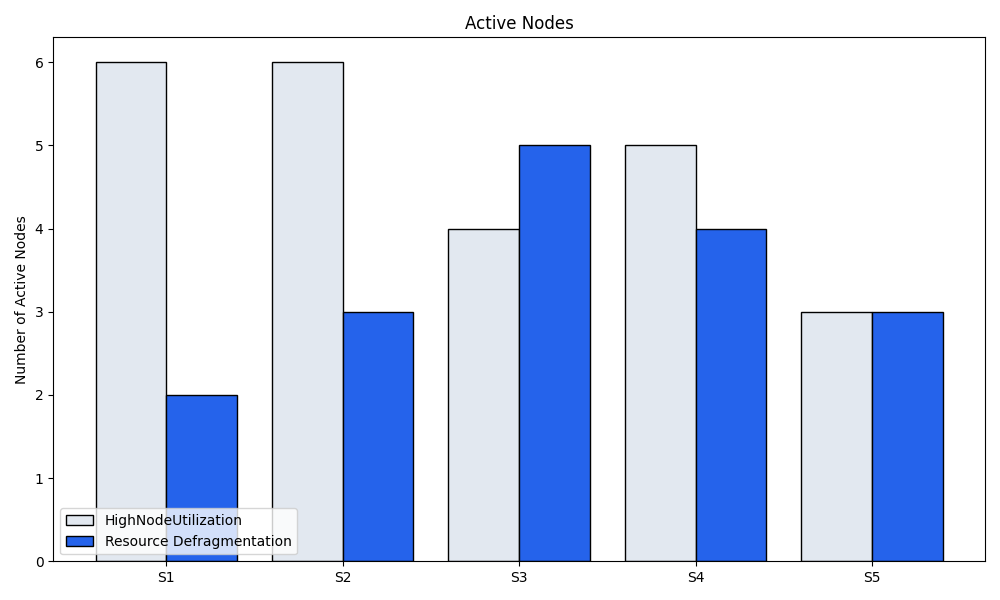
\includegraphics[width=0.95\textwidth]{assets/pics/defrag/chart_active_nodes.png}
    \caption{Active worker Nodes per scenario after descheduling.}
    \label{fig:defrag_active_nodes}
\end{figure*}

ResourceDefragmentation reclaims four Nodes in S1 and three in S2, while HNU performs no eviction in either scenario, as shown in Figure \ref{fig:defrag_active_nodes}. HNU requires Nodes above its threshold to act as packing targets; uniformly low or uniformly fragmented layouts therefore produce no action. ResourceDefragmentation instead treats sparse Nodes and low bin-quality Nodes as resource-only consolidation sources, then uses \textit{predictSchedulerTarget} to choose Pods with feasible denser targets even when the baseline cannot form high- and low-utilization groups.

S3 is the only reclamation case won by HNU. Dense balanced targets already exist, allowing the threshold policy to drain two Nodes greedily. ResourceDefragmentation respects the \(0.90\) ceiling and reclaims one Node. S5 is especially useful because both policies reclaim the same Node, allowing placement quality and eviction cost to distinguish them.

The consolidation effect is also visible in the density of the surviving Nodes. Figure \ref{fig:defrag_avg_utilization} reports the average active-Node utilization \(\bar{U}\) after descheduling: in the consolidation and fragmentation scenarios ResourceDefragmentation drives the retained Nodes to substantially higher density than HNU, confirming that the reclaimed capacity is absorbed rather than left uniformly sparse.

\begin{figure*}[tbp]
    \centering
    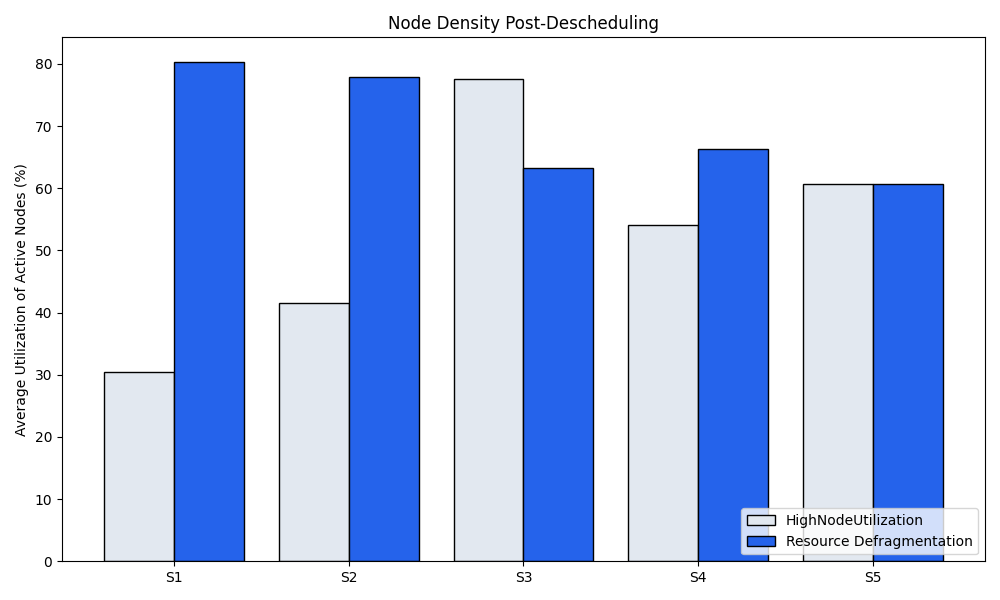
\includegraphics[width=0.95\textwidth]{assets/pics/defrag/chart_avg_utilization.png}
    \caption{Average utilization of active Nodes after descheduling (\(\bar{U}\)).}
    \label{fig:defrag_avg_utilization}
\end{figure*}

\subsection{Stranding Reduction}
\label{sec:defrag_stranding_results}

\begin{table*}[tbp]
    \centering
    \caption{Cluster Stranding Score Before and After Descheduling}
    \label{tab:defrag_stranding}
    \renewcommand{\arraystretch}{1.2}
    \begin{tabular}{@{}l c c@{}}
        \hline
        \textbf{Scenario} & \textbf{HighNodeUtilization} & \textbf{ResourceDefragmentation} \\
        \hline
        S1 & \(0.049 \rightarrow 0.049\) & \(0.049 \rightarrow 0.050\) \\
        S2 & \(3.727 \rightarrow 3.727\) & \(3.727 \rightarrow \mathbf{0.971}\) \\
        S3 & \(1.395 \rightarrow 1.408\) & \(1.395 \rightarrow \mathbf{1.386}\) \\
        S4 & \(3.243 \rightarrow 3.243\) & \(3.243 \rightarrow \mathbf{1.112}\) \\
        S5 & \(1.338 \rightarrow 1.298\) & \(1.338 \rightarrow \mathbf{0.123}\) \\
        \hline
    \end{tabular}
\end{table*}

\begin{figure*}[tbp]
    \centering
    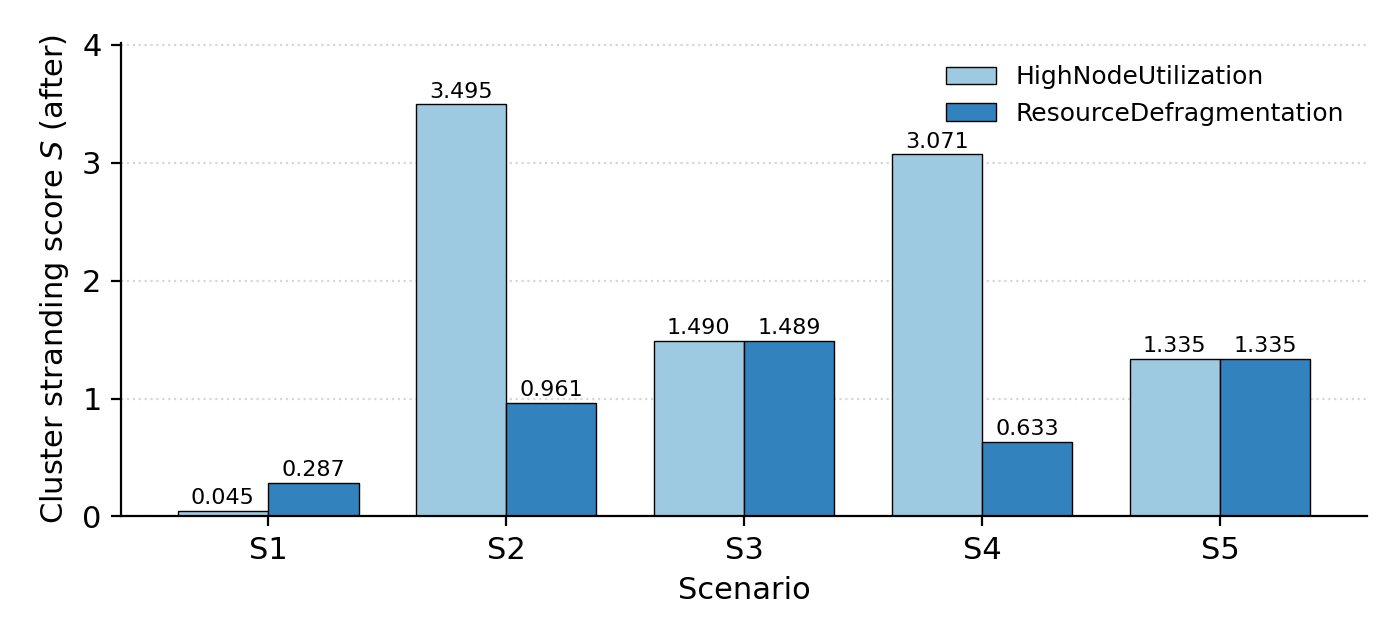
\includegraphics[width=0.95\textwidth]{assets/pics/defrag/chart_stranding.png}
    \caption{Final cluster stranding score \(S\) per scenario (lower is better).}
    \label{fig:defrag_stranding}
\end{figure*}

As summarized in Figure \ref{fig:defrag_stranding}, the result separates node reclamation from dimensional defragmentation. S1 begins with little stranding, so packing four Nodes into two leaves \(S\) essentially unchanged. In S2 and S4, ResourceDefragmentation uses the predicted-target score to combine complementary shapes and reduces \(S\) by approximately \(74\%\) and \(66\%\), respectively; HNU does not act.

In S3, HNU reclaims one additional Node but slightly worsens \(S\), whereas ResourceDefragmentation reduces it from \(1.395\) to \(1.386\). This shows the consequence of retaining resource shape in the target objective rather than optimizing Node count alone.

\subsection{S5 Heterogeneous-Drain Analysis}
\label{sec:defrag_s5_analysis}

S5 tests whether the selector distinguishes Pods on the same source Node by the shape of their predicted destinations. The source contains CPU-heavy and memory-heavy candidates, while other active Nodes expose complementary residual capacity.

ResourceDefragmentation predicts a feasible target for each candidate and compares projected target bin scores after applying the ceiling and pack-upward guards. It moves the CPU-shaped Pod to the Node with spare CPU-compatible balance and the memory-shaped Pod to the complementary Node. The source becomes empty after two evictions, and the receiving Nodes end in nearly balanced states. Consequently, \(S\) falls from \(1.338\) to \(0.123\), a reduction of approximately \(91\%\).

HNU also empties one Node, but it requires three evictions and only reduces \(S\) to \(1.298\). Thus, equal Node reclamation does not imply equal defragmentation quality. The predicted-target criterion produces both a better placement and lower disruption.

\subsection{Headroom and Eviction Efficiency}
\label{sec:defrag_headroom_efficiency}

\begin{table*}[tbp]
    \centering
    \caption{Balanced Headroom and Eviction Count}
    \label{tab:defrag_headroom_efficiency}
    \renewcommand{\arraystretch}{1.2}
    \begin{tabular}{@{}l c c c c@{}}
        \hline
        \textbf{Scenario} & \textbf{HNU \(H_{balanced}\)} & \textbf{HNU Evict.} & \textbf{RD \(H_{balanced}\)} & \textbf{RD Evict.} \\
        \hline
        S1 & \(42\) & \(0\) & \(39\) & \(10\) \\
        S2 & \(15\) & \(0\) & \(\mathbf{29}\) & \(6\) \\
        S3 & \(18\) & \(4\) & \(\mathbf{19}\) & \(2\) \\
        S4 & \(13\) & \(0\) & \(\mathbf{24}\) & \(5\) \\
        S5 & \(32\) & \(3\) & \(\mathbf{38}\) & \(\mathbf{2}\) \\
        \hline
    \end{tabular}
\end{table*}

\begin{figure*}[tbp]
    \centering
    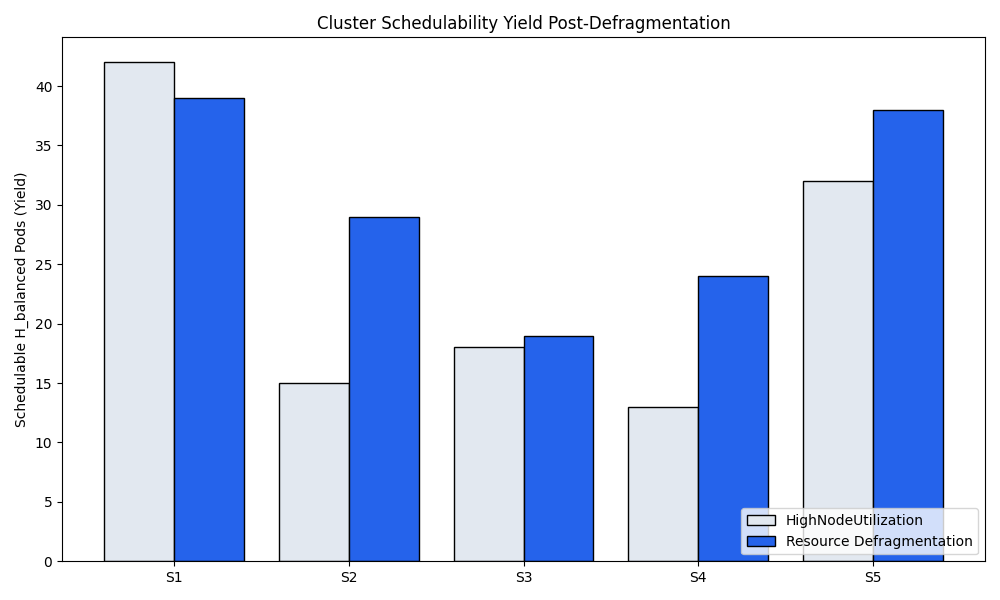
\includegraphics[width=0.95\textwidth]{assets/pics/defrag/chart_h_balanced.png}
    \caption{Balanced headroom \(H_{balanced}\) per scenario after descheduling.}
    \label{fig:defrag_h_balanced}
\end{figure*}

HNU retains higher distributed headroom in S1 because it leaves all six Nodes active; this is not a node reclamation success. In the fragmentation scenarios, ResourceDefragmentation exposes substantially more balanced headroom, as shown in Figure \ref{fig:defrag_h_balanced}. S5 is the strongest efficiency result: two ResourceDefragmentation evictions reclaim one Node, reduce \(S\) by \(1.215\), and leave headroom for 38 balanced reference Pods. HNU uses three evictions for the same reclamation, reduces \(S\) by only \(0.040\), and leaves headroom for 32 reference Pods.

The eviction cost behind these gains is reported in Figure \ref{fig:defrag_evictions}. ResourceDefragmentation spends evictions only where consolidation or defragmentation is achievable, and in S3 and S5 it reaches an equal or better cluster state than HNU with fewer Pod movements.

\begin{figure*}[tbp]
    \centering
    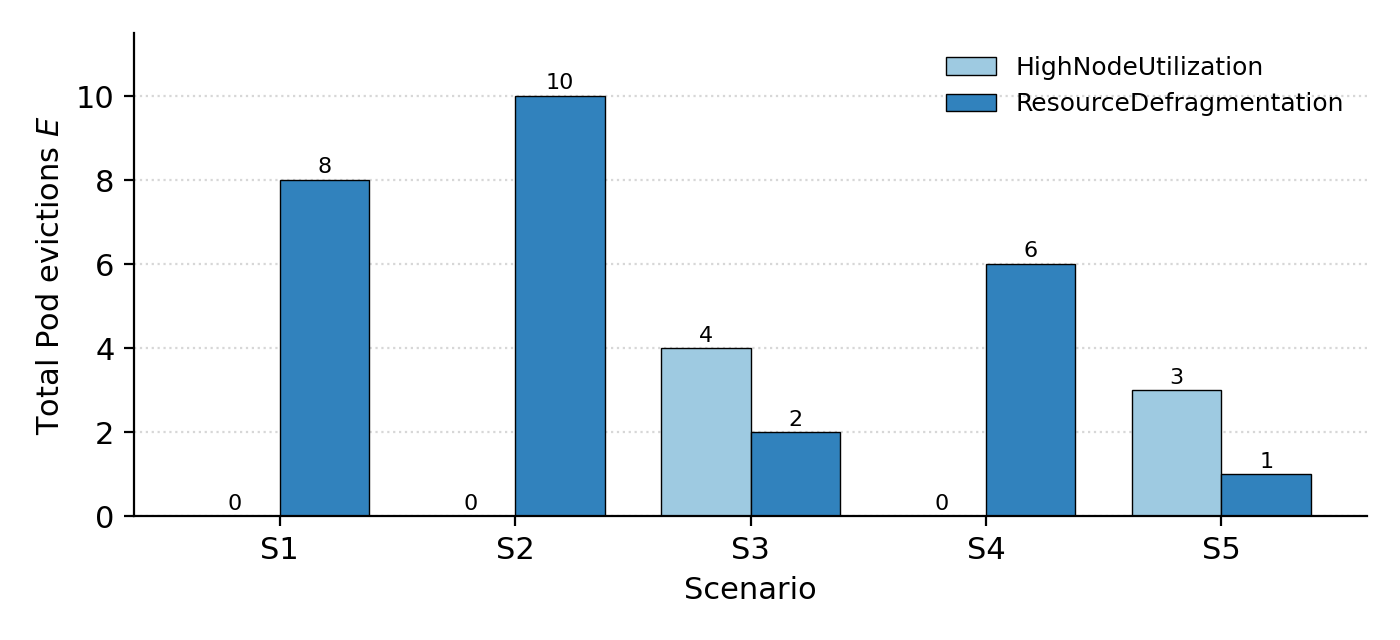
\includegraphics[width=0.95\textwidth]{assets/pics/defrag/chart_evictions.png}
    \caption{Total Pod evictions per scenario (\(E_{count}\)).}
    \label{fig:defrag_evictions}
\end{figure*}

\subsection{Shape-Specific Schedulability Yield}
\label{sec:defrag_shape_headroom}

Balanced headroom alone does not show \emph{which} kind of workload a defragmented layout can still admit. To make this explicit, the residual capacity is also probed with three skewed reference Pods: a CPU-skewed Pod, a memory-skewed Pod, and a large jumbo Pod (\(800\,m/324\,Mi\)). Table \ref{tab:defrag_shape_headroom} reports the resulting yields after descheduling.

\begin{table*}[tbp]
    \centering
    \caption{Schedulability Yield by Reference-Pod Shape After Descheduling}
    \label{tab:defrag_shape_headroom}
    \small
    \renewcommand{\arraystretch}{1.2}
    \begin{tabular}{l cc cc cc}
        \hline
        & \multicolumn{2}{c}{\textbf{CPU-skewed}} & \multicolumn{2}{c}{\textbf{Memory-skewed}} & \multicolumn{2}{c}{\textbf{Jumbo}} \\
        \textbf{Scenario} & \textbf{HNU} & \textbf{RD} & \textbf{HNU} & \textbf{RD} & \textbf{HNU} & \textbf{RD} \\
        \hline
        S1 & \(12\) & \(\mathbf{13}\) & \(12\) & \(\mathbf{13}\) & \(6\) & \(\mathbf{8}\) \\
        S2 & \(9\)  & \(9\)          & \(9\)  & \(\mathbf{11}\) & \(0\) & \(\mathbf{6}\) \\
        S3 & \(\mathbf{6}\) & \(5\)   & \(6\)  & \(\mathbf{9}\)  & \(\mathbf{4}\) & \(2\) \\
        S4 & \(4\)  & \(\mathbf{8}\)  & \(4\)  & \(\mathbf{7}\)  & \(3\) & \(\mathbf{4}\) \\
        S5 & \(\mathbf{12}\) & \(11\) & \(11\) & \(11\)          & \(6\) & \(\mathbf{7}\) \\
        \hline
    \end{tabular}
\end{table*}

In the fragmentation scenarios, ResourceDefragmentation increases the yield for skewed and jumbo workloads where it matters most. In S2 and S4, where complementary CPU-heavy and memory-heavy Nodes are merged, it lifts memory-skewed yield (\(9 \to 11\) in S2, \(4 \to 7\) in S4) and restores jumbo capacity that the baseline cannot provide at all in S2 (\(0 \to 6\)), as shown in Figures \ref{fig:defrag_h_cpu_skewed}, \ref{fig:defrag_h_mem_skewed}, and \ref{fig:defrag_h_jumbo}. In S5 it matches or slightly exceeds the baseline on every shape while using fewer evictions.

The two cases where HNU leads, CPU-skewed and jumbo yield in S3, reflect the same trade-off seen in the balanced headroom and stranding results: HNU empties an additional Node by greedily packing onto pre-dense targets, which leaves more whole-Pod slots free but at a slightly worse stranding score. ResourceDefragmentation instead preserves resource shape, so its remaining capacity is more evenly balanced across dimensions rather than concentrated on one emptied Node.

\begin{figure*}[tbp]
    \centering
    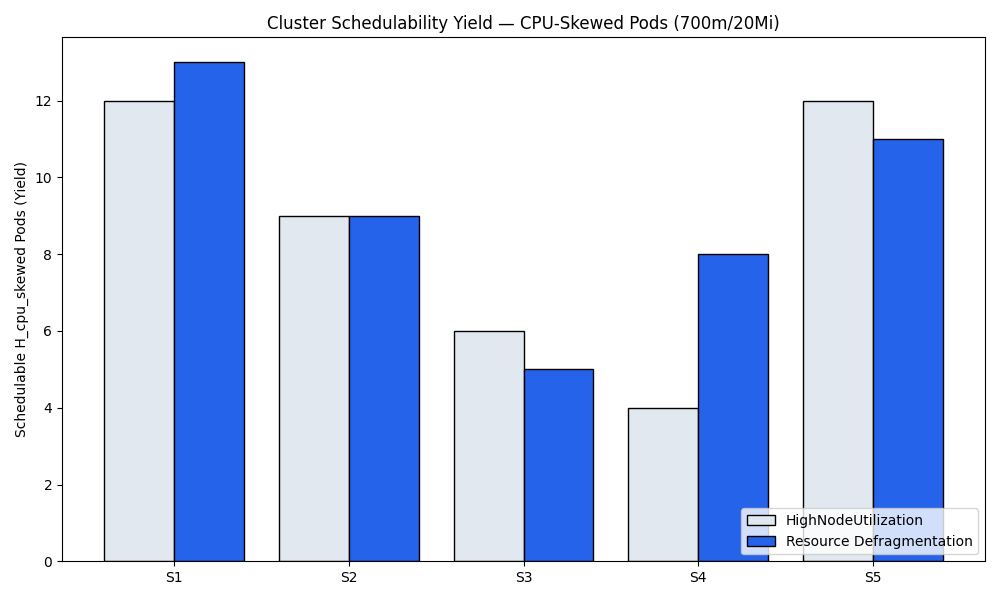
\includegraphics[width=0.95\textwidth]{assets/pics/defrag/chart_h_cpu_skewed.png}
    \caption{CPU-skewed schedulability yield \(H_{cpu\text{-}skewed}\) per scenario after descheduling.}
    \label{fig:defrag_h_cpu_skewed}
\end{figure*}

\begin{figure*}[tbp]
    \centering
    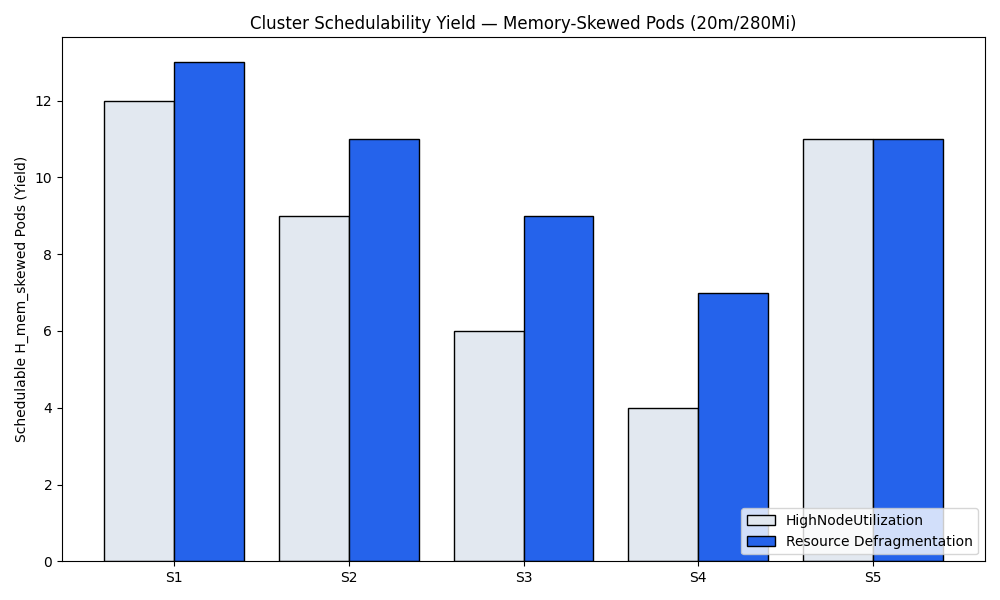
\includegraphics[width=0.95\textwidth]{assets/pics/defrag/chart_h_mem_skewed.png}
    \caption{Memory-skewed schedulability yield \(H_{mem\text{-}skewed}\) per scenario after descheduling.}
    \label{fig:defrag_h_mem_skewed}
\end{figure*}

\begin{figure*}[tbp]
    \centering
    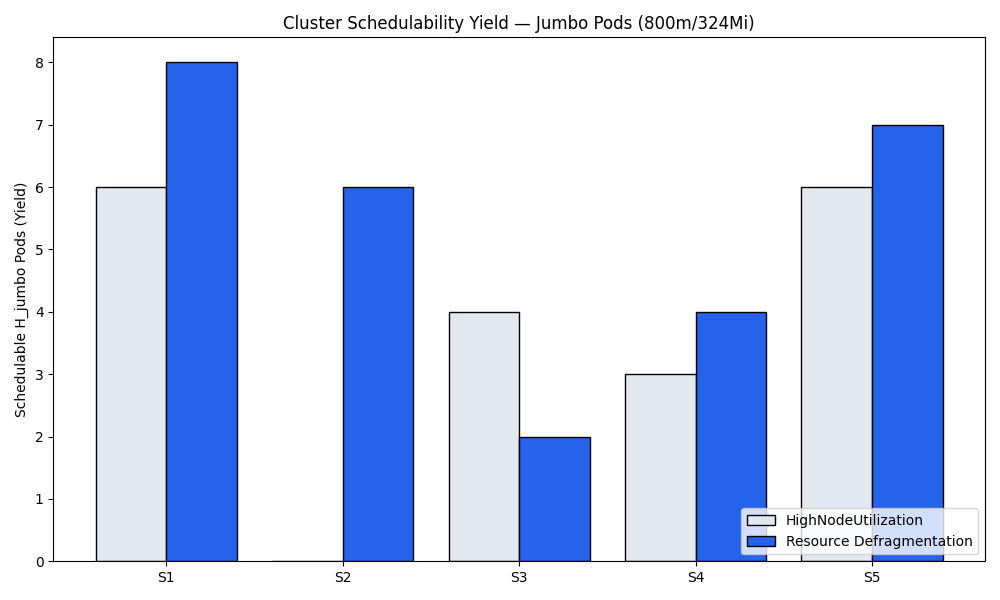
\includegraphics[width=0.95\textwidth]{assets/pics/defrag/chart_h_jumbo.png}
    \caption{Jumbo (\(800\,m/324\,Mi\)) schedulability yield \(H_{jumbo}\) per scenario after descheduling.}
    \label{fig:defrag_h_jumbo}
\end{figure*}

\subsection{Convergence and Safety}
\label{sec:defrag_convergence_safety}

\begin{table*}[tbp]
    \centering
    \caption{Representative Per-Pass Eviction Counts}
    \label{tab:defrag_convergence}
    \begin{tabular}{@{}l c c@{}}
        \hline
        \textbf{Scenario} & \textbf{HighNodeUtilization} & \textbf{ResourceDefragmentation} \\
        \hline
        S1 & \(0\) & \(8, 2, 0\) \\
        S2 & \(0\) & \(6, 0\) \\
        S3 & \(4, 0\) & \(2, 0\) \\
        S4 & \(0\) & \(4, 1, 0\) \\
        S5 & \(3, 0\) & \(2, 0\) \\
        \hline
    \end{tabular}
\end{table*}

Every scenario converges to a zero-eviction pass within two or three passes, with no oscillation. Across all repetitions, no after-snapshot contains a Pending Pod. All evicted Pods are controller-owned and eligible under the default evictor, infrastructure namespaces are excluded, and no eviction request remains outstanding. These observations validate the feasibility guard, target ceiling, and bounded execution loop.

\subsection{Resource Policy Findings}
\label{sec:defrag_findings}

The evaluation yields four main findings:

\begin{itemize}
    \item ResourceDefragmentation consolidates uniformly underutilized and uniformly fragmented layouts in which HNU is a no-op.
    \item ResourceDefragmentation reduces dimensional stranding in S2, S4, and S5 while preserving or increasing balanced schedulability headroom.
    \item Predicted-target bin-score selection is especially effective for heterogeneous drain Nodes, reducing S5 stranding from \(1.338\) to \(0.123\) with two evictions.
    \item The policy converges without leaving Pods Pending, showing that node reclamation pressure can be combined with explicit feasibility and utilization guards.
\end{itemize}

%-----------------------------------------------------------------------------%
\section{Conclusion and Future Work}
\label{bab:5}
%-----------------------------------------------------------------------------%

This research designed and evaluated \textit{ResourceDefragmentation}, a request-based Kubernetes Descheduler \textit{Balance} policy that repairs post-placement CPU-memory fragmentation without replacing the kube-scheduler.

\textbf{Identifying fragmented Nodes.} \textit{ResourceDefragmentation} identifies fragmented Nodes directly from their request-space resource shape, without relying on runtime usage or a single utilization threshold. It selects drain candidates from average utilization and CPU-memory bin quality, orders them by the Resource Imbalance Index (RII) and Free-Space Index (FSI), and then evicts the Pod whose predicted landing Node, found through \textit{predictSchedulerTarget}, has the best projected bin score. A target ceiling and pack-upward guard prevent overfilling a Node or relocating a workload to an emptier one. Together the drain ordering, predicted-target criterion, and guards drive effective packing while keeping eviction churn low.

\textbf{Effectiveness against the baseline.} ResourceDefragmentation reclaimed four Nodes in S1, two in S2, and one in S4, all cases where \textit{HighNodeUtilization} performed no eviction. It cut dimensional stranding by \(73\%\) in S2 (\(3.495 \to 0.961\)) and \(79\%\) in S4 (\(3.071 \to 0.633\)) in the layouts where stranding is reducible, and on the already-irreducible layouts (S3, S5) it correctly declined unproductive evictions rather than churning. Four of five scenarios converged within three passes and no run left a Pod Pending.

\textbf{Component attribution.} An ablation that disabled one mechanism at a time showed that each earns its place on a different axis: RII/FSI ordering preserves stranding quality (removing it regressed S4 from \(0.633\) to \(1.581\)), the pack-upward guard bounds eviction churn (removing it roughly doubled evictions for no stranding gain), and the projected-bin-score selector lowers the eviction count without changing the converged stranding. The stranding wins therefore come from the consolidation-and-defragmentation pipeline as a whole, while the selector keeps disruption low.

Overall, the results support a simple conclusion: selecting eviction candidates by the balance of their predicted landing Nodes, combined with request feasibility, bounded utilization, drain ordering, and pack-upward behavior, is enough to drive useful Node reclamation and dimensional defragmentation where it is achievable while avoiding wasteful eviction where it is not.

\subsection{Future Work}
\label{sec:future_works}

\begin{itemize}
    \item \textbf{Broader Resource Dimensions:} Extend the framework to additional resource dimensions, including storage and GPU, so that target prediction and bin-quality scoring can handle workloads beyond CPU and memory.
    \item \textbf{Scheduler Coordination:} Establish and evaluate scheduler coordination mechanisms that expose the predicted target, or a compatible scoring signal, to the kube-scheduler, ensuring that predicted-target placements align with actual scheduling decisions and eliminating the misalignment that currently bounds maximum defragmentation precision.
    \item \textbf{Pending-Pod Awareness:} Introduce Pending-pod awareness into the eviction pipeline so that drain candidates are selected with knowledge of already-unschedulable workloads, ensuring evictions free the right resource type on the right Node to unblock Pending Pods rather than delaying them further.
    \item \textbf{Threshold Sensitivity Analysis:} Conduct a sensitivity analysis of the drain threshold, target ceiling, and related parameters across various workloads and cluster types to characterize their effect on node reclamation, stranding reduction, and convergence stability.
    \item \textbf{Broader Generalizability Evaluation:} Evaluate the plugin across broader cluster shapes, node heterogeneity, and workload mixes to assess generalizability beyond the five scenarios studied.
    \item \textbf{Broader Baselines and Multi-Seed Runs:} Extend the comparison beyond \textit{HighNodeUtilization} once faithful reference implementations of prior pseudocode-only proposals become available, and repeat each policy-scenario cell across multiple seeds to quantify run-to-run variation.
\end{itemize}


\bibliographystyle{apalike}
\bibliography{config/references}

\clearpage
\onecolumn
\appendix
\section{Resource Defragmentation Balance Filter Algorithm}
\label{appendix:resource_defrag}
\lstinputlisting[
    caption={ResourceDefragmentation predicted-target eviction workflow.},
    label={lst:resource_defrag},
]{assets/codes/pseudos/resource-defrag.psu}

\end{document}
